% Created 2019-05-18 Sat 14:48
% Intended LaTeX compiler: pdflatex
\documentclass[10pt,oneside,x11names]{article}
\usepackage[utf8]{inputenc}
\usepackage[T1]{fontenc}
\usepackage{graphicx}
\usepackage{grffile}
\usepackage{longtable}
\usepackage{wrapfig}
\usepackage{rotating}
\usepackage[normalem]{ulem}
\usepackage{amsmath}
\usepackage{textcomp}
\usepackage{amssymb}
\usepackage{capt-of}
\usepackage{hyperref}
\usepackage{geometry}
\usepackage{palatino}
\usepackage{siunitx}
\usepackage{braket}
\usepackage[euler-digits,euler-hat-accent]{eulervm}
\author{Brian Beckman, Uri Ran}
\date{\textit{<2015-11-23 Mon>}}
\title{Uri's SM in Lisp: Version 0.0.5}
\hypersetup{
 pdfauthor={Brian Beckman, Uri Ran},
 pdftitle={Uri's SM in Lisp: Version 0.0.5},
 pdfkeywords={},
 pdfsubject={},
 pdfcreator={Emacs 26.2 (Org mode 9.2.2)},
 pdflang={English}}
\begin{document}

\maketitle
\setcounter{tocdepth}{2}
\tableofcontents


\section{Preliminaries}
\label{sec:org972d939}

\begin{verbatim}
Emacs version: GNU Emacs 26.2 (build 2, x86_64-pc-linux-gnu, GTK+ Version 3.24.4)
 of 2019-04-12
org version: 9.2.2
\end{verbatim}


This is version 0.0.5 of Uri Ran's State-Machine demo.

\subsection{How to Use this Document}
\label{sec:org78b2f78}

This is a literate program. Code and documentation cohabit a single
``org-mode'' file called \texttt{sm.org}. You must use emacs org-mode and org-babel to
process the file. If you're a VIM user, use \emph{Spacemacs}\footnote{\url{http://spacemacs.org}}, a
near-perfect emulation of VIM in emacs. The file is plain text, however, and
you may edit it with elementary tools.

Typeset the document by running the emacs command \texttt{org-latex-export-to-pdf}.
See section \ref{section:running_code_directly}, Running Code Directly for
instructions on running the code inside emacs or spacemacs.

Extract or ``tangle'' the code from this document via emacs command
\texttt{org-babel-tangle} or \texttt{C-c C-v t}. Run extracted code in practically any
implementation of Common Lisp. In this document, we demonstrate running the
code in SBCL[TODO:ref] and ECL[TODO:ref].

\section{Vertex Struct}
\label{sec:org6a6959a}

A \emph{vertex} or ``state'' in a state-machine diagram has an \emph{entry action}, a
\emph{do-action}, an \emph{exit-action}, and an \emph{event table}. We prefer the word
``vertex'' to avoid overloading the word ``state.'' An \emph{edge} that connects two
vertices has a \emph{guard} function and a \emph{transition} or \emph{edge function}. Edges
are one-way, or \emph{directed}. A state machine may have cycles.

A state machine may \emph{inhabit} exactly one vertex at any time. Visualize the
dynamics of the machine as a sequence of steps in which the token either stays
within the current vertex or moves from one vertex to another. Each step is a
response to an \emph{event} or \emph{input}. Events or inputs are denoted by \emph{symbols}
drawn from a finite \emph{alphabet}, one at a time.
Consider a unique, global variable or \emph{token} called \texttt{*current-vertex*}. The
value of this token represents the vertex that the state machine currently inhabits.

The entry action of a vertex runs whenever the \texttt{*current-vertex*} token enters
that vertex. The exit action of a vertex runs whenever the \texttt{*current-vertex*}
token leaves that vertex.

Do-actions concern \emph{polling}, not further discussed here. Although we define
do-actions here, we don't use them; they're a placeholder in this version.

\subsection{Running the Machine}
\label{sec:orgdbb9b3f}
\label{section:running}

The \emph{event table} of a vertex is an associative lookup table (or dictionary)
from event symbols to a list of \emph{triples}. When an event symbol arrives, its
corresponding triple is looked up. Each triple has a \emph{guard function}, an
\emph{edge-action}, and a new vertex. The engine will \texttt{funcall} the guard function
in the list, in the order they're presentated, and accept the transition if
the guard returns \texttt{t}, which means \emph{true} in Lisp. ``Accepting the transition''
means running the edge action and moving the token to the new vertex if the
new vertex is non-nil (TODO: what if the new vertex is \emph{nil}?). The exit
action of the old vertex runs first, then the edge action, and then the entry
action of the new vertex. If the guard does not return \texttt{t}, the engine logs a
trace message and does nothing.

The following lisp code defines the vertex struct.

\begin{verbatim}
(defstruct vertex-t name entry-ac do-ac exit-ac evt-tbl)
\end{verbatim}

\texttt{defstruct} gives us default constructors and accessors. That's all we need
for this demonstration. Should we need more in the future, consider
\texttt{defclass}.

As a side-effect of calling \texttt{defstruct}, Lisp defines the following functions
in our environment

\begin{itemize}
\item \texttt{(make-vertex-t}
\begin{itemize}
\item \texttt{:name} \emph{<name your vertex>}
\item \texttt{:entry-ac} \emph{<put a function value here>}
\item \texttt{:do-ac} \emph{<put another function value>}
\item \texttt{:exit-ac} \emph{<put another function value>}
\item \texttt{:evt-tbl} \emph{<put an event table, here>} \texttt{)}
\item produces an instance of \texttt{vertex-t}; this is a \emph{constructor} function
\end{itemize}

\item \texttt{(vertex-t-name} \emph{<some instance of vertex-t>} \texttt{)} produces the name of the
vertex; this is like the dot notation in C / C++, \emph{i.e.}, like \texttt{someInstance.name}

\item \texttt{(vertex-t-entry-ac} \emph{<some instance of vertex-t>} \texttt{)} produces the
entry-action function value of the vertex; also like dot, just for a
different instance variable

\item \texttt{(vertex-t-do-ac} \emph{<some instance of vertex-t>} \texttt{)} produces the
do-action function value of the vertex; ditto

\item \texttt{(vertex-t-exit-ac} \emph{<some instance of vertex-t>} \texttt{)} produces the
exit-action function value of the vertex; etc.

It's possible to mutate the \emph{instance variables} of a \texttt{defstruct}, but we
don't need to do so here.
\end{itemize}

\section{Utilities}
\label{sec:orga482ae2}

\subsection{Boolean fair coin}
\label{sec:org9d6db9e}

\begin{verbatim}
(defun coin () (= 0 (random 2)))
\end{verbatim}

\subsection{LINQ}
\label{sec:org04e7a96}

The following are convenience functions for manipulating lists. They are
derived from \texttt{LINQ} (Language Integrated Query) [TODO: reference?]. Find a
separate and independent unit test for these functions in the directory of
this project [TODO: bring unit tests into this literate program.

\begin{verbatim}
(defun take (seq n)
  "(take seq n) gives the first n elements of the seq. (take seq -n) gives the
  last n elements of the seq. This works on strings as well."
  (check-type seq sequence)
  (check-type n integer)
  (let ((l (length seq)))
    (cond ((>= n 0) (subseq seq 0 (min n l)))
          ((<  n 0) (subseq seq (max 0 (+ n l)) l))
          ((=  n 0) (subseq seq 0 0)))))

(defun drop (seq n)
  "(drop seq n) gives the seq with the first n elements removed. (drop seq -n)
  gives the seq with the last n elements removed. This works on strings as
  well."
  (let ((l (length seq)))
    (check-type seq sequence)
    (check-type n integer)
    (cond ((>= n 0) (subseq seq (min n l) l))
          ((<  n 0) (subseq seq 0 (max 0 (+ n l))))
          ((=  n 0)  seq))))

(defun str-last (str)
  "(str-last non-empty-string) produces the last character in a non-empty
  string."
  (check-type str string)
  (let ((l (length str)))
    (assert (> l 0))
    (subseq str (- l 1) l)))
\end{verbatim}

\subsection{Drawing to DOT}
\label{sec:org0841290}

Borrowed from ``Land of Lisp'' by Conrad Barski, M.D. [TODO: reference]

\subsubsection{{\bfseries\sffamily TODO} Robustify}
\label{sec:org94d5c5c}

a-la \url{http://tinyurl.com/y63ugo} and \url{http://tinyurl.com/j23lakq}

\begin{verbatim}
(defparameter *max-label-length* 30)
\end{verbatim}

\begin{verbatim}
(defun dot-name (exp)
  (substitute-if #\_ (complement #'alphanumericp) (prin1-to-string exp)))

(defun dot-label (exp)
  (if exp
      (let ((s (write-to-string exp :pretty nil)))
        (if (> (length s) *max-label-length*)
            (concatenate 'string (subseq s 0 (- *max-label-length* 3)) "...")
            s))
      ""))

(defun nodes->dot (nodes)
  (mapc (lambda (node)
          (fresh-line)
          (princ (dot-name (car node)))
          (princ "[label=\"")
          (princ (dot-label node))
          (princ "\"];"))
        nodes))

(defun edges->dot (edges)
  (mapc (lambda (node)
          (mapc (lambda (edge)
                  (fresh-line)
                  (princ (dot-name (car node)))
                  (princ "->")
                  (princ (dot-name (car edge)))
                  (princ "[label=\"")
                  (princ (dot-label (cdr edge)))
                  (princ "\"];"))
                (cdr node)))
        edges))

(defun dgraph->dot (nodes edges)
  (princ "digraph{")
  (nodes->dot nodes)
  (edges->dot edges)
  (princ "}"))

(defun uedges->dot (edges)
  (maplist (lambda (lst)
             (mapc (lambda (edge)
                     (unless (assoc (car edge) (cdr lst))
                       (fresh-line)
                       (princ (dot-name (caar lst)))
                       (princ "--")
                       (princ (dot-name (car edge)))
                       (princ "[label=\"")
                       (princ (dot-label (cdr edge)))
                       (princ "\"];")))
                   (cdar lst)))
           edges))

(defun ugraph->dot (nodes edges)
  (princ "graph{")
  (nodes->dot nodes)
  (uedges->dot edges)
  (princ "}"))

(defun dot->png (fname thunk)
  (with-open-file (*standard-output* (concatenate 'string fname ".dot") :direction :output :if-exists :supersede)
    (funcall thunk))
  ;; (ext:shell (concatenate 'string "dot -Tpng -O " fname ".dot"))
  )

(defun dgraph->png (fname nodes edges)
  (dot->png fname
            (lambda ()
              (dgraph->dot nodes edges))))

(defun ugraph->png (fname nodes edges)
  (dot->png fname
            (lambda ()
              (ugraph->dot nodes edges))))
\end{verbatim}

\section{Action and Guard Functions}
\label{sec:org89ab90d}

\subsection{Actions}
\label{sec:orgae32bb5}

\subsubsection{{\bfseries\sffamily TODO} Parameters or return values for actions?}
\label{sec:orgc8adaf4}

\subsubsection{{\bfseries\sffamily TODO} Contexts for actions and guards}
\label{sec:org5a40965}

\subsubsection{Vertex Actions}
\label{sec:org3f140f9}

For \emph{entry}, \emph{polling} (currently undefined) and \emph{exit}, respectively.

Our example actions just print to standard output because this is just a
demo. They might have arbitrary side effects.

\begin{verbatim}
(defun vertex-1-entry () (print "vertex 1 entry"))
(defun vertex-2-entry () (print "vertex 2 entry"))
(defun vertex-3-entry () (print "vertex 3 entry"))
(defun vertex-4-entry () (print "vertex 4 entry"))

(defun vertex-1-do    () (print "vertex 1 do"))
(defun vertex-2-do    () (print "vertex 2 do"))
(defun vertex-3-do    () (print "vertex 3 do"))
(defun vertex-4-do    () (print "vertex 4 do"))

(defun vertex-1-exit  () (print "vertex 1 exit"))
(defun vertex-2-exit  () (print "vertex 2 exit"))
(defun vertex-3-exit  () (print "vertex 3 exit"))
(defun vertex-4-exit  () (print "vertex 4 exit"))
\end{verbatim}

\subsubsection{Edge Actions}
\label{sec:org0fba3d2}

When the engine takes a transition, moving the token from one vertex to
another, it runs these functions.

\begin{verbatim}
(defun act-a    () (print "action a" ))
(defun act-b    () (print "action b" ))
(defun act-c    () (print "action c" ))
(defun act-d    () (print "action d" ))
(defun act-na   () (print "action na"))
(defun act-self () (print "self-transition action"))
\end{verbatim}

\subsection{Guards (Boolean-Valued)}
\label{sec:org4e105af}

Here are some made-up functions for our example.

\begin{verbatim}
(defun guard-x     () (coin) )
(defun guard-y     () (coin) )
(defun guard-z     () (coin) )
(defun guard-true  () t      )
(defun guard-false () nil    )
(defun guard-na    () t      )
\end{verbatim}

\section{The Diagram}
\label{sec:orgddb6a6b}

If \texttt{nym} is \texttt{foo}, we want functions \texttt{foo-entry}, \texttt{foo-do}, and \texttt{foo-exit}
automatically assigned. The following macro, \texttt{defvertex}, expands into this
boilerplate and makes an instance of \texttt{vertex-t} named \texttt{*foo*}. The name of
the instance is a global \emph{special variable} demarcated with asterisks, aka
earmuffs. Special variables are global. Lisp has distinctions between
special variables and other kinds of globals. These distinctions do not
concern us here.\footnote{\url{http://www.flownet.com/ron/specials.pdf}}

\texttt{defvertex} works by defining strings for \texttt{foo-entry}, \texttt{foo-do}, \texttt{foo-exit}
when \texttt{nym} is \texttt{foo}; \texttt{bar-entry}, etc., when \texttt{nym} is \texttt{bar}, and so on.
\texttt{defvertex} converts the strings to Lisp symbols, then writes new code that
defines \texttt{*foo*} and the related functions.

\subsection{How to Define a Vertex}
\label{sec:orgf21cc51}

\begin{verbatim}
(defparameter *vertices* nil)
(defmacro defvertex (nym evt-tbl)
  (let* ((dynvar (format nil "*~A*"     nym)) ;; "format nil" means
         (entry  (format nil "~A-entry" nym)) ;; "write to a string"
         (doo    (format nil "~A-do"    nym))
         (exit   (format nil "~A-exit"  nym))
         (vtxsym (with-input-from-string (s dynvar) (read s))))
    `(progn
       (defparameter ,vtxsym
         (make-vertex-t
          :name     (format nil "~A" ,nym)
          :entry-ac (function ,(with-input-from-string (s entry) (read s)))
          :do-ac    (function ,(with-input-from-string (s doo  ) (read s)))
          :exit-ac  (function ,(with-input-from-string (s exit ) (read s)))
          :evt-tbl  ,evt-tbl))
       (push ,vtxsym *vertices*))))
\end{verbatim}

\subsection{Vertices in Our Example Diagram}
\label{sec:org2bb3a77}

The new vertices in the event table are unevaluated symbols. That's because we
want to refer to them before they're defined. We know their names at the time
we write the table, but they don't always have values. This is a good way to
avoid forward referencing and resolution.

\begin{verbatim}
(defvertex "vertex-1"
    '((ev-2 (guard-true act-c    *vertex-3* ))
      (ev-3 (guard-x    act-self *vertex-1* ))  ))
(defvertex "vertex-2"
    '((ev-4 (guard-true act-na   *vertex-1* ))
      (ev-6 (guard-x    act-c    *vertex-4* ))  ))
(defvertex "vertex-3"
    '((ev-1 (guard-x    act-na   nil        )
            (guard-y    act-b    *vertex-1* )
            (guard-z    act-na   *vertex-1* ))
      (ev-5 (guard-na   act-d    *vertex-4* ))  ))
(defvertex "vertex-4"
    '((ev-3 (guard-y    act-d    *vertex-2* ))
      (ev-6 (guard-x    act-c    *vertex-3* ))  ))
\end{verbatim}

\subsection{Drawing The Diagram}
\label{sec:org40d5a36}

\begin{verbatim}
(defparameter *wizard-nodes*
  '((v1 1)
    (v2 2)
    (v3 3)
    (v4 4)))

(defparameter *wizard-edges*
  '((v1 (v3 g-t  ev-2)
        (v1 g-x  ev-3))
    (v2 (v1 g-t  ev-4)
        (v4 g-x  ev-6))
    (v3 (v1 g-y  ev-1)
        (v1 g-z  ev-1)
        (v4 g-na ev-5))
    (v4 (v2 g-y  ev-3)
        (v3 g-x  ev-6))))
\end{verbatim}

\begin{verbatim}
(dgraph->png "wizard" *wizard-nodes* *wizard-edges*)
\end{verbatim}

\begin{verbatim}
dot -Tpng -O wizard.dot
\end{verbatim}
\begin{center}
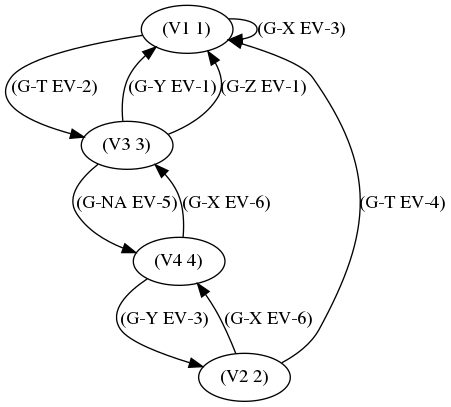
\includegraphics[width=.9\linewidth]{wizard.dot.png}
\end{center}

\subsection{Simulating Transitions in the Diagram}
\label{sec:org7455244}

\subsubsection{The Vertex Token}
\label{sec:org619d162}

At any time, the state machine is ``in'' a vertex. This means that the value
of \texttt{*current-vertex*} is the currently inhabited vertex instance. We call
\texttt{*current-vertex*} the \emph{vertex token}. Visualize a token on a gaming board
moving from one vertex to another.

\begin{verbatim}
(defparameter *current-vertex* *vertex-1*)
\end{verbatim}

\subsubsection{The Engine}
\label{sec:org572be1f}

\begin{enumerate}
\item Eval-First-Admissible-Triple
\label{sec:org48ef1eb}

This function implements the token-moving strategy discussed in section
\ref{section:running} above and returns the current value of the token
\texttt{*current-vertex*}, whether it's changed or not.

When the new-vertex is \texttt{nil}, the \texttt{*current-vertex*} does not change and the
action functions do not run, even if the guard is true. That is not the
same as a transition-to-self, during which the action functions \emph{do} run.
Our example machine has one self-transition: from \texttt{*vertex-1} to
\texttt{*vertex-1} when \texttt{ev-3} arrives.

\begin{verbatim}
(defun eval-first-admissible-triple (triples)
  (cond (triples
         (let* ((triple     (first  triples))
                (guard      (first  triple))
                (action     (second triple))
                (new-vertex (eval (third  triple))))
           (if (and (funcall guard) new-vertex)
               (progn
                 (funcall (vertex-t-exit-ac *current-vertex*))
                 (funcall action)
                 (setf *current-vertex* new-vertex)
                 (funcall (vertex-t-entry-ac *current-vertex*)))
               (progn
                 (format t "~%~A: guard failed; trying next guard"
                         (vertex-t-name *current-vertex*))
                 (eval-first-admissible-triple (rest triples))))))
        (t (format t "~%~A: all guards failed; doing nothing"
                   (vertex-t-name *current-vertex*))))
  *current-vertex*)
\end{verbatim}

\item SM-Engine
\label{sec:org02238b7}

This takes an event symbol, does lookup in the diagram, and performs the
indicated transition.

\begin{verbatim}
(defun sm-engine (event-symbol)
  (let ((line (rest (assoc event-symbol
                           (vertex-t-evt-tbl *current-vertex*)))))
    (if line
        (eval-first-admissible-triple line)
        (progn ;; else
          (format t "~%~A: event ~W not found; doing nothing"
                  (vertex-t-name *current-vertex*)
                  event-symbol)
          *current-vertex*)))) ;; return current vertex in this case

\end{verbatim}
\end{enumerate}

\section{Running the Code}
\label{sec:orgdc907c0}

This document contains live code. You can run the code in two ways:
inside org mode or by extracting (tangling) the code and running it at the
command line.

\subsection{Setting up Two Good Lisps}
\label{sec:orgdc61aa7}

Install SBCL (Steel Bank Common Lisp)[TODO:ref] for running this code in the
editor or a REPL, and ECL (Embeddable Common Lisp)[TODO:ref] for generating C
code. On a mac, this is trivial with homebrew:

\begin{itemize}
\item \texttt{brew install sbcl}

\item \texttt{brew install ecl}
\end{itemize}

It's also trivial on Ubuntu Linux:

\begin{itemize}
\item \texttt{sudo apt install sbcl}

\item \texttt{sudo apt install ecl}
\end{itemize}

You will need SLIME in Emacs or Spacemacs to run the code in this file
directly. To find out whether you have slime, type \texttt{M-x slime}. If you don't
have it, get it.

\subsection{Running Code Directly}
\label{sec:org6d87dd3}
\label{section:running_code_directly}

Once you have SLIME running in Emacs, type \texttt{M-x slime} to start the REPL,
then type \texttt{M-x org-babel-execute-buffer} or \texttt{C-c C-v b} to run all the code
in this file. At the very end of this file, you will see a few unit tests.
Put the cursor in that code block and type \texttt{C-c C-c} repeatedly to run the
unit tests over and over. The results will be slightly different each time
because the guard functions flip coins.

\subsection{Extracting Code From This File}
\label{sec:orgc9bd7fc}

Type \texttt{M-x org-babel-tangle} or \texttt{C-c C-v t} and you should get a file named
\texttt{sm.lisp}. Run it in SBCL as follows:

\begin{itemize}
\item \texttt{sbcl -{}-load sm.lisp}
\end{itemize}

\subsection{Generating, Inspecting, Running C code}
\label{sec:orgd49eb13}

After extracting code, run ECL at the command prompt:
\begin{verbatim}
$ ecl -load make.lisp
\end{verbatim}
Watch all the messages, then type
\begin{verbatim}
(quit)
\end{verbatim}
to leave the ECL REPL, then
\begin{verbatim}
$ ./sm
\end{verbatim}
to run the generated code. You should see exactly the same output as you
would get from the last section below.

\subsubsection{{\bfseries\sffamily TODO} Create Deeply Embedded C}
\label{sec:orgb117c91}

The generated code is in the files \texttt{sm.c}, \texttt{sm.h}, and \texttt{sm.data}. The
generated code just calls the ECL runtime kernel. This is a
\emph{shallow embedding} of lisp in C. A \emph{deep embedding} would write C code that
bypasses lisp-specific helpers and more directly express the model. Bypassing
a lisp runtime means that we can avoid garbage collection and other hazards
in the lisp implementation.

A good way to produce a deep embedding will be through macros.  The deeply
embedded code should be comparable to the code that Uri wrote by hand.

\subsection{Interactively}
\label{sec:org944f6bf}

To run in an external REPL, paste the following code into the REPL (and
remove the quote, of course). Don't run this code in emacs; it will deadlock
as emacs and the program contend over the terminal.

\begin{verbatim}
'(load "sm.lisp")
'(let ((ev 1024))
  (loop while (> ev 0) do
    (format t "~%Enter an event number > 0, 0 to quit: ")
    (setf ev (read))
    (format t "~%~A: searching for event ~A"
            (vertex-t-name *current-vertex*)
            (format nil "ev-~A" ev))
    (if (numberp ev)
        (progn
          (with-input-from-string (s (format nil "ev-~A" ev))
               (sm-engine (read s nil 0))))
        (format t "~%~A: failure: type-of ev wasn't a number, but a ~A"
                (vertex-t-name *current-vertex*)
                (type-of ev)))))

\end{verbatim}

\subsection{Unit Tests, Exhaustive Tests}
\label{sec:org0f85a34}

Because the current guards are random, exhaustively testing them isn't as
trivial as enumeration.

Run the following unit test repeatedly; it can be a little different each
time, but the machine should always end up in vertex 3.

\begin{verbatim}
(print (equal *current-vertex* *vertex-1*))
(print (eq *current-vertex* *vertex-1*))
(print (eq (sm-engine 'ev-1) *vertex-1*))
(print (eq (sm-engine 'ev-4) *vertex-1*))
(print (eq (sm-engine 'bogus) *vertex-1*))
(print (eq (sm-engine 'ev-3) *vertex-1*))
(print (eq (sm-engine 'ev-2) *vertex-3*))
\end{verbatim}

\begin{verbatim}

T
T
vertex-1: event EV-1 not found; doing nothing
T
vertex-1: event EV-4 not found; doing nothing
T
vertex-1: event BOGUS not found; doing nothing
T
vertex-1: guard failed; trying next guard
vertex-1: all guards failed; doing nothing
T
"vertex 1 exit"
"action c"
"vertex 3 entry"
T
\end{verbatim}
\end{document}
